\documentclass[a4paper,14pt]{article} 
\usepackage{lscape}
%%% Страница
\usepackage{extsizes} % Возможность сделать 14-й шрифт
\usepackage{geometry} % Простой способ задавать поля
        \geometry{top=25mm}
        \geometry{bottom=30mm}
        \geometry{left=30mm}
        \geometry{right=20mm}
 %

\usepackage[T1,T2A]{fontenc}
\usepackage[utf8]{inputenc}
\usepackage[english,russian]{babel}
\usepackage{amssymb,amsmath}
\usepackage{float}
\usepackage[unicode, pdftex]{hyperref}
\usepackage[europeanresistors,americaninductors]{circuitikz}
\usetikzlibrary{calc}
\usepackage[T1,T2A]{fontenc}
\usepackage[utf8]{inputenc}

\usepackage{amssymb,amsmath}
\usepackage{float}
\usepackage[unicode, pdftex]{hyperref}
\usepackage{booktabs}
\usepackage{multirow}

\usepackage{tikz}
\usepackage{rotating}
%\usepackage[landscape]{geometry}
\usepackage{graphicx}
\graphicspath{{pictures/}}
\DeclareGraphicsExtensions{.pdf,.png,.jpg}
\usepackage{pgfplots}
\usepackage{wrapfig}
\usepackage{rotating}
\usepackage{lipsum}
\usepackage{nccmath}
\usepackage{caption}
\usepackage{siunitx}
%\usepackage[american,cuteinductors,smartlabels]{circuitikz}
%\usepackage[backend=biber]{biblatex}

\usepackage[]{hyperref}
\ctikzset{bipoles/thickness=1}
\ctikzset{bipoles/length=0.8cm}
\ctikzset{bipoles/diode/height=.375}
\ctikzset{bipoles/diode/width=.3}
\ctikzset{tripoles/thyristor/height=.8}
%\ctikzset{tripoles/thyristor/width=1}
\ctikzset{tripoles/thyristor/width=0.8}
\ctikzset{bipoles/vsourceam/height/.initial=.7}
\ctikzset{bipoles/vsourceam/width/.initial=.7}
\tikzstyle{every node}=[font=\small]
\tikzstyle{every path}=[line width=0.8pt,line cap=round,line join=round]

\ctikzset{resistor = european}
\ctikzset{inductor = american}
\ctikzset{tripoles/thyristor/height=0.55}
\ctikzset{tripoles/thyristor/height 2=0.4}
%\ctikzset{tripoles/thyristor/width=0.35} 
\ctikzset{tripoles/thyristor/diode width left=0.35}
\ctikzset{tripoles/thyristor/diode width right=0.35}

\ctikzset{bipoles/cuteindictor/coils/.initial=3}
\ctikzset{bipoles/americanindictor/coils/.initial=3}
\ctikzset{bipoles/cuteindictor/coils/.initial=3}
\ctikzset{bipoles/americanindictor/coils/.initial=3}
\hypersetup{
colorlinks=false,
}
\usepackage{textcomp}

\begin{document}
%METHODICAL INSTRUCTIONS FOR PERFORMING LABORATORY WORKS

\section{Study of a step-up (boost) pulse-width DC-DC converter}

\subsection{Objective}

The study of electromagnetic processes, external, regulatory and energy characteristics of a boost pulse-width converter constant voltage.


\subsection{Lab Description}

In this laboratory work are used: ``Stand power module''/<<Модуль питания стенда>>/ (single-phase), modules ``DC-DC Converters''/ <<Преобразователи постоянного напряжения>>/, ``Meter power''/ <<Измеритель мощности>>, ``Load''/ <<Нагрузка>>/ (single-phase) and two-channel oscilloscope.

Front panel of the ``DC/DC Converter'' module shown in fig. \ref{ris1}. As a series (step-down voltage) the key is a diagram of the converter 071, and as a parallel (up) key


%DC CONVERTERS
\begin{figure}[!ht]
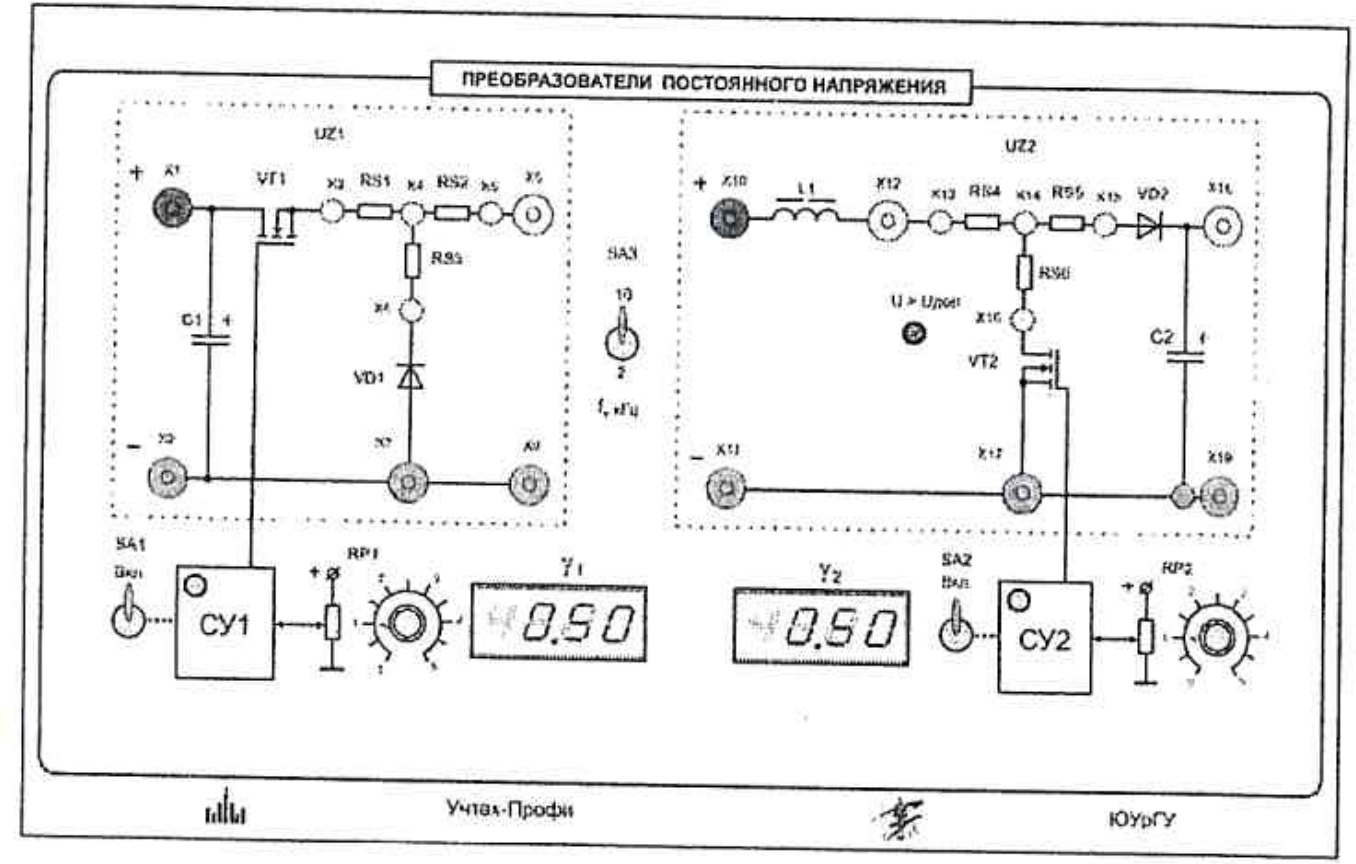
\includegraphics[scale=0.35]{img_60}
	\caption{The front panel of the module "DC-DC Converters".}
	\label{ris1}
\end{figure}

The serial key is turned on by the toggle switch $SA1$, with this lights up the LED control panel $\textcyrillic{СУ}1$. 
Duty cycle is adjustable by potentiometer $RP1$ and displayed on a nearby 4-bit indicator. 
Similarly, $SA2$ and $RP2$ control the parallel key. 
If the key voltage exceeds the permissible voltage, the LED lights up
$U> U_\textcyrillic{доп}$ ($>U_{perm}$).  The frequency of the switching keys is determined by the position of the toggle switch $SA3$. All shunts $RS1$ -- $RS6$ with a resistance of 1 Ohm are designed to take waveforms of currents.





\subsection{The task}

\begin{enumerate}

\item Assemble the circuit in accordance with fig. 2.1.
\item Take the waveforms of currents and voltages on the circuit elements for the given parameters.
\item Take the control $U_L=F(\gamma)$ and energy $P_d=F(\gamma)$, $P_L=F(\gamma)$, $\eta=F(\gamma)$, $q_{ripple}=F(\gamma)$ characteristics of the converter 
at a constant value of the load resistance $R_L$ and the given $U_d$ and carrier frequency $f_{carrier}$.
\item Take the external $U_L =F(I_L)$ and energy $P_d = F(I_L)$, $P_L=F(I_L)$, $\eta=F(I_L)$, 
$q_{ripple}=F(I_L)$ characteristics with the duty cycle $\gamma$ for given $U_d$ and $f_{carrier}$.
\item Investigate the influence of the carrier frequency $f$ on the ripple coefficient $q_{ripple}$ of the voltage 
	at the load $u_L$.
\end{enumerate}

\subsection{Initial data}

The base point (mode) for which the waveforms are taken and through which the recorded characteristics pass:

\begin{tabular}{ll}
	carrier frequency 	&	$f=2$ kHz;\\
	ducy cycle 		& 	$\gamma = 0.6$;\\
	power supply voltage 	& 	$U_d = 15$ V; \\
	load current 		& 	$I_L = 80$ mA.
\end{tabular}

\noindent The base point can be changed as instructed by the teacher.

\subsection{Guidelines}

\begin{enumerate}
	\item 
		Assemble the circuit for the study of the DC-DC converter in accordance with Fig. \ref{ris2}
Additional external connections are indicated by dashed lines.

Set the given carrier frequency $f_{carrier}$ with the $SA3$ toggle switch.
Set potentiometer knobs $RP1$, $RP2$ to position <<0>>.
Set the handle of the load current regulator $RP$ in the ``Load''(<<Нагрузка>>) module (Н) to the <<0>> position 
corresponding to the minimum load current (maximum load resistance).



\begin{figure}[!ht]
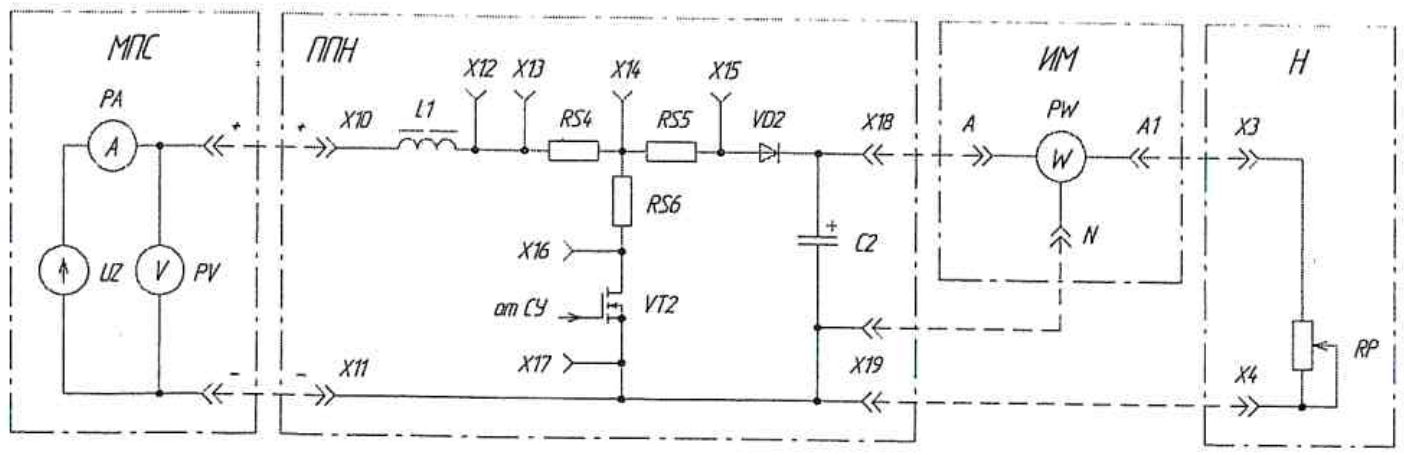
\includegraphics[scale=0.3]{img_61}
\caption{Schematic diagram for the study of a step-up DC-DC converter}
	\label{ris2}
\end{figure}

%Fig. 2.1. Schematic diagram for the study of a step-up DC-DC converter.





Turn on the automatic switch $ОF1$ ``Stand power module''/<<Модуль питания стенда>> (МПС).

Switch on the ``Grid''/<<Сеть>> toggle switch of the ``Power Meter''/<<Изме\-ри\-тель мощности>> module.
To transfer the ``Power Meter''/<<Измеритель мощности>> module to the mode of measuring constant currents and voltages, 
simultaneously press the ``P/Q/S'' and ``$f$/$\cos \varphi$/$\varphi$'' buttons.
Keep the buttons pressed until ``DC''/<<Постоянный ток>> appears on the display.
Set measurement limits: toggle switch <<U>> 300 V, toggle switch <<I>> 0.2 A.

Toggle switch $SA1$ to turn on the power of the control system 
		of the ``DC/DC Converter''/<<Преобразователь постоянного напряжения>> module.

Switch on the power supply toggle switch $SA2$ in the ``Stand power module''/МПС module, 
and using the potentiometer $RP1$ set the set voltage of the power supply.

\item Take the waveforms of currents and voltages on the circuit elements for the given parameters.

\begin{enumerate}
\item take the waveforms of the voltage on the transistor switch $u_{VT}$ and the current through the transistor $i_{VT}$.
To do this, check the set value of the supply voltage $U_d$ and set the set value of the ducy cycle $\gamma$ 
		with the handle of the potentiometer $RP2$ (basic mode).
Using the knob of the current regulator $RP$, set the set value of the load current $I_L$.
Connect the channel $CH1$ of the oscilloscope to the $RS6$ shunt (``input''  -- socket $X14$, 
the oscilloscope case ``$\bot$'' -- socket $X16$), 
		and the input of channel $CH2$ -- to socket $X17$ (voltage on the transistor key).
To obtain a positive voltage deviation $u_{VT}$, press the $CH2$ $INV$ button on the oscilloscope.

\noindent{\bf Attention: hereinafter, before taking the oscillograms, check the position of the zero line by moving the switch mode of the input inputs of the amplifiers ``AC-GND-DC'' to the position ``GND''.
		This line is first plotted on the waveform.}

Draw from the oscilloscope screen the waveform. Define scales by voltage, current and time;

\item to take an oscillogram of the current consumed from the $i_d$ power source at the same given values $U_d$, 
$\gamma$ and $I_L$.
To do this, connect the oscilloscope channel $CH1$ to the $RS4$ shunt (``input'' -- socket $X13$, 
oscilloscope housing ``$\bot$'' -- socket $X14$). Draw the waveform, save the scale;

\item take the waveforms of the voltage on the diode $u_D$ and the current through the diode $i_D$ at the same given values $U_d$,
$\gamma$ and $I_L$. To do this, connect the oscilloscope channel $CH1$ to the $RS4$ shunt (``input'' -- socket $X14$, 
the oscilloscope housing ``$\bot$'' -- socket $X15$), and the channel input $CH2$ -- to socket $X18$.
To obtain a positive voltage deviation $u_D$, press the $CH2$ $INV$ button on the oscilloscope.
Draw the oscillogram from the oscilloscope screen, save the scale;

\item to take a waveform of the voltage at the load $u_L$ at the same given values $U_d$, $\gamma$ and $I_L$.
To do this, connect the oscilloscope housing ``$\bot$'' to socket $X19$, and the input of channel $CH2$ to socket $X18$.
Draw the oscillogram from the oscilloscope screen, save the scale.
\end{enumerate}

\item Take the control $U_L = F(\gamma)$ and energy $P_d = F(\gamma)$, $P_L=F (\gamma)$, $\eta=F(\gamma)$, 
$q_{ripple} = F(\gamma)$ characteristics of the converter with a constant value of the load resistance $R_L$ and given $U_d$ 
and $f_{carrier}$. Set basic mode.
Determine $R_L$ by the formula

$$
R_L = \frac{U_L}{I_L}
$$

By changing the $\gamma$ with the handle of the potentiometer $RP2$ in the range from 0.1 to 0.8, observe the current $I_d$ and voltage $U_L$. They should not exceed respectively 1 A and 100 V.
Record the readings of the $U_d$, $I_d$, $U_L$, $I_L$, $P_L$ devices, and also using an oscilloscope to measure the amplitude of the voltage ripple on the $U_L$ load.
To do this, switch the oscilloscope channel $CH1$ to the open input ``AC'' (variable component of the input signal).
Measure the double amplitude of the ripple voltage on the $U_L$ load.
Populate the measurements into table 2.1.
Mark the transition point from continuous to intermittent (boundary current).
%\end{enumerate}

Table 2.1

\begin{tabular}{l|p{10pt}|p{10pt}|p{10pt}|p{10pt}|p{10pt}|p{10pt}|p{100pt}}
        $gamma$ & &&&&&& notes\\
        \cmidrule{1-8}
        $U_d$, V &&&&&&&\multirow{9}{*}{\begin{minipage}{0.3\textwidth}$\gamma=$, $f_{carrier}=$ \end{minipage}}\\
        \cmidrule{1-7}
        $I_d$, A &&&&&&\\
        \cmidrule{1-7}
$U_L$, V &&&&&&\\
        \cmidrule{1-7}
        $I_L$, A &&&&&&\\
        \cmidrule{1-7}
        ${\scriptstyle \Delta}U_L, V$&&&&&&\\
        \cmidrule{1-7}
	$q_{ripple}$ &&&&&&\\
        \cmidrule{1-7}
$P_d$,W &&&&&&\\
        \cmidrule{1-7}
$P_L$,W &&&&&&\\
        \cmidrule{1-7}
$\eta$&&&&&&\\
\end{tabular}

Energy indicators calculated by the following formulas:

input power
\begin{equation}
	P_d = U_d\cdot I_d
\end{equation}
Efficiency
\begin{equation}
	\eta = \frac{P_L}{P_d}
\end{equation}
ripple ratio at load
\begin{equation}
q_{ripple} \approx \frac{\Delta U_L}{2U_L} 
\end{equation}

Repeat measurements with another, for example, twice as high load resistance $R_L$.

The characteristics for different $R_L$ values are built in the same axes.
Graphs for $P_d$ and $P_L$ capacities, build on the same axis;

\item Take the external $U_L=F(I_L)$ and energy $P_d = F(I_L)$, $P_L = F(I_L)$, $\eta = F(I_L)$, $q_{ripple} = F(I_L)$ 
characteristics with duty cycle $\gamma$ for given $U_d$ and $f_{carrier}$.
To do this, set the set duty cycle $\gamma$ with potentiometer $RP1$.
Changing the load resistance with a rheostat $RP$, record the readings $U_d$, $I_d$, $U_L$, $I_L$, $P_L$, $U_L$,
$\Delta U_L$.  in table 2.2.

Repeat measurements with a different $\gamma$ value, for example, $\gamma = 0.5$.

The characteristics for different $\gamma$ values are built in the same axes.
Graphs for $P_d$ and $P_L$ capacities, build on the same axis.

\item To study the influence of the carrier frequency $f_{carrier}$ on the ripple coefficient 
$q_{ripple}$ of the voltage at the load for the basic mode.

Set the basic mode and determine the ripple coefficient $q_{ripple}$ of the voltage at the load.
Switch the toggle switch $SA3$ to another position and again determine the ripple factor $q_{ripple}$ 
at a different carrier frequency $f_{carrier}$.

Turn off the toggle switch $SA2$ of the power supply of the ``DC/DC Converter'' module, and then the automatic machine 
$QF1$ of the “Power module of the stand”.

Table 2.2


\begin{tabular}{l|p{10pt}|p{10pt}|p{10pt}|p{10pt}|p{10pt}|p{10pt}|p{100pt}}
        $R_L$ Ohm& &&&&&& notes\\
        \cmidrule{1-8}
        $U_d$, V &&&&&&&\multirow{9}{*}{\begin{minipage}{0.3\textwidth}$\gamma=$, $f_{carrier}=$ \end{minipage}}\\
        \cmidrule{1-7}
        $I_d$, A &&&&&&\\
        \cmidrule{1-7}
$U_L$, V &&&&&&\\
        \cmidrule{1-7}
        $I_L$, A &&&&&&\\
        \cmidrule{1-7}
        ${\scriptstyle \Delta}I_L, A$&&&&&&\\
        \cmidrule{1-7}
        $q_{ripple}$ &&&&&&\\
        \cmidrule{1-7}
$P_d$,W &&&&&&\\
        \cmidrule{1-7}
$P_L$,W &&&&&&\\
        \cmidrule{1-7}
$\eta$&&&&&&\\
\end{tabular}

\end{enumerate}
 

\subsection{Report content}

The report should contain the following items:

\begin{itemize}
	\item the name and purpose of the work;

	\item initial data, circuit diagram of the installation;

	\item processed waveforms;

	\item the results of experimental studies and the calculations performed on them, placed in the corresponding tables;

	\item constructed characteristics (regulatory, external and energy);



	\item conclusions on the work:
		\begin{itemize}
			\item explain the effect of the gamma duty cycle on the load voltage of the boost DC-DC converter;

			\item explain the influence of the fill factor y on the efficiency of the step-up DC-DC converter;

			\item explain the effect of the carrier frequency f on the ripple factor of the voltage q.
		\end{itemize}
\end{itemize}

\subsection{Control questions}

\begin{itemize}
	\item What are the components of power loss in key mode?

	\item What is the control characteristic of a step-up DC-DC converter? What kind does she have?

	\item What is the external characteristic of a step-up DC-DC converter? What kind does she have?

	\item How to determine the coefficient of ripple voltage on the load?

	\item What is affected by a change in carrier frequency?

	\item How to determine the efficiency of a DC / DC converter?

	\item How to take the waveforms of currents and voltages in the circuit?

	\item How to connect the inputs of two-channel oscillography of currents and voltages?
\end{itemize}
\end{document}
